\documentclass{standalone}
\usepackage{tikz}
\usepackage{ctex,siunitx}
\setCJKmainfont{Noto Serif CJK SC}
\usepackage{tkz-euclide}
\usepackage{amsmath}
\usetikzlibrary{patterns, calc}
\usetikzlibrary {decorations.pathmorphing, decorations.pathreplacing, decorations.shapes,}
\newcommand\dynanometer[3][0]{
  \begin{scope}[#2,rotate=#1,inner sep=0pt]
    \coordinate (A) at (0,2.0);
    \coordinate (B) at (0,2.0+#3*0.2);
    \foreach \x/\y in {100/2.0, 70/1.5, 50/1.2, 30/0.7 }
    {
      \draw[line width=\y pt,gray!\x ]([yshift=1cm]B)circle(0.2);
    }
    \fill[top color=gray, bottom color=gray,middle color=white]([xshift=-1mm,yshift=7mm]B)rectangle([xshift=1mm,yshift=8.7mm]B);
    \fill[green!30!black]([xshift=2.8mm,yshift=6mm]B)--([xshift=2.8mm,yshift=-1.2cm]B)to[bend left=50]([xshift=-2.8mm,yshift=-1.2cm]B)--([xshift=-2.8mm,yshift=6mm]B)to[bend left=50]cycle;
    \fill[lightgray,even odd rule](0.1,0.4)arc(360:180:0.1)--++(0,1.6)--++(0.2,0)--cycle(0,0.4)circle(0.05)([xshift=-0.4mm]A)rectangle++(0.8mm,0.5mm);
    \fill[lightgray!30,even odd rule]([xshift=2.2mm,yshift=5mm]B)--([xshift=2.2mm,yshift=-1.1cm]B)to[bend left]([xshift=-2.2mm,yshift=-1.1cm]B)[rounded corners=2pt]--([xshift=-2.2mm,yshift=5mm]B)[sharp corners]--([xshift=-1mm,yshift=5mm]B)arc(180:0:0.1)[rounded corners=2pt]--cycle[sharp corners]
    ([xshift=-0.4mm,yshift=2mm]B)rectangle([xshift=0.4mm]A);
    \draw[darkgray](0.1,0.1)arc(360:90:0.1)--++(0,0.15);
    \foreach \x in {0,1,...,9}
    {
      \draw[line width=0.1pt,line join=round,lightgray]([yshift=2mm-\x*0.15mm-\x*#3*0.2mm]B)--++(0.3mm,-0.0375mm-#3*0.05mm)--++(-0.6mm,-0.075mm-#3*0.1mm)--++(0.3mm,-0.0375mm-#3*0.05mm);
    }
    \fill[red]([yshift=-0.2mm]A)--([xshift=-1mm]A)--([xshift=1mm]A);
    \foreach \x in {0,1,2,3,4}
    {
      \draw[ultra thin]([xshift=0.5mm,yshift=-\x*2mm]B)--++(0.07,0)node[rotate=#1,right]{\resizebox{!}{0.5mm}{\x}};
      \draw[ultra thin]([xshift=-0.5mm,yshift=-\x*2mm]B)--++(-0.07,0)node[rotate=#1,left]{\resizebox{!}{0.5mm}{\x}};
      \foreach \y in {1,2,3,4,6,7,8,9}
      {
        \draw[ultra thin]([xshift=0.5mm,yshift=-\x*2mm-\y*0.2mm]B)--++(0.05,0);
        \draw[ultra thin]([xshift=-0.5mm,yshift=-\x*2mm-\y*0.2mm]B)--++(-0.05,0);
      }
      \draw[ultra thin]([xshift=0.5mm,yshift=-\x*2mm-1mm]B)--++(0.06,0);
      \draw[ultra thin]([xshift=-0.5mm,yshift=-\x*2mm-1mm]B)--++(-0.06,0);
    }
    \draw[ultra thin]([xshift=0.5mm,yshift=-1cm]B)--++(0.07,0)node[rotate=#1,right]{\resizebox{!}{0.5mm}{5}};
    \draw[ultra thin]([xshift=-0.5mm,yshift=-1cm]B)--++(-0.07,0)node[rotate=#1,left]{\resizebox{!}{0.5mm}{5}};
  \end{scope}
  }
\begin{document}
\small
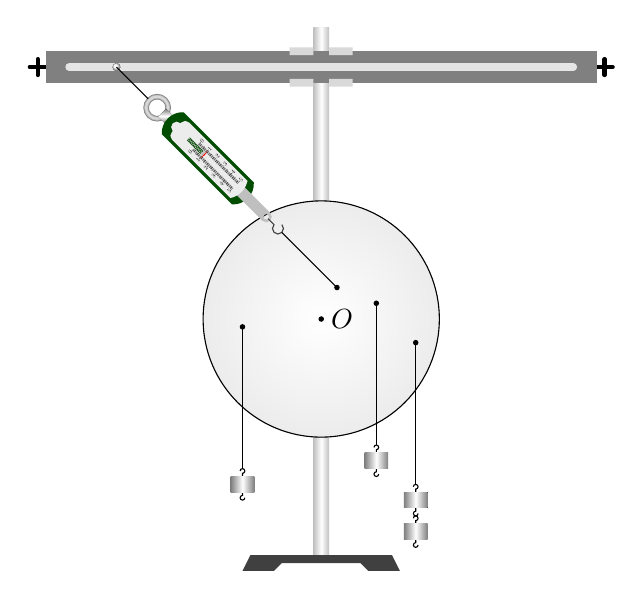
\begin{tikzpicture}[>=latex,scale=1]
  \fill[left color=lightgray,right color=lightgray,middle color=white](-0.1,-3)rectangle(0.1,3.7);
  \fill[darkgray](-0.9,-3)--(-1,-3.2)--(-0.6,-3.2)--(-0.5,-3.1)--(0.5,-3.1)--(0.6,-3.2)--(1,-3.2)--(0.9,-3)--cycle;
  \fill[outer color=lightgray!30,inner color=white,draw](0,0)circle(1.5);
  \dynanometer[45]{xshift=-5mm,yshift=11mm,scale=0.7}{1}
  \draw(-0.5,1.1)--(0.2,0.4);
  \fill(0,0)circle(1pt)node[right]{$O$}(0.2,0.4)circle(1pt)(0.7,0.2)circle(1pt)(1.2,-0.3)circle(1pt)(-1.0,-0.1)circle(1pt);
  \foreach  \x/\y in {0.7/0.2,1.2/-0.3,-1/-0.1}
  {
    \draw(\x,\y)--++(0,-1.8);
    \draw(\x-0.03,\y-1.83)arc(180:-90:0.03)--++(0,-0.28)arc(90:360:0.03);
    \fill[left color=gray, right color=gray,middle color=white](\x-0.15,\y-1.9)rectangle++(0.3,-0.2);
  }
  \draw(1.17,-2.53)arc(180:-90:0.03)--++(0,-0.28)arc(90:360:0.03);
  \fill[left color=gray, right color=gray,middle color=white](1.05,-2.6)rectangle++(0.3,-0.2);
  \draw[line cap=round,ultra thick](-3.7,3.2)--(3.7,3.2)(-3.6,3.1)--(-3.6,3.3)(3.6,3.1)--(3.6,3.3);
  \fill[gray](-3.5,3.4)rectangle(3.5,3.0);
  \fill[lightgray!60](0.1,3.45)rectangle(0.4,3.35)(0.1,2.95)rectangle(0.4,3.05)(-0.1,3.45)rectangle(-0.4,3.35)(-0.1,2.95)rectangle(-0.4,3.05);
  \draw[line width=1mm, line cap=round,lightgray!40](-3.2,3.2)--(3.2,3.2);
  \fill[ball color=white](-2.6,3.2)circle(0.05);
  \draw(-2.6,3.2)--++(-45:0.57);
\end{tikzpicture}
\end{document}